% Emacs, this is -*-latex-*-
\documentclass[12pt]{ugentreport}
\usepackage[a4paper]{geometry}
\geometry{a4paper,margin=3cm,marginparwidth=20mm}
\usepackage[dutch]{babel}
\usepackage{parskip}
\usepackage{amsfonts}
\usepackage{amsmath}
\usepackage{cancel}
\usepackage{commath}
\usepackage{amssymb}
\usepackage{parskip}
\usepackage{rotating}
\usepackage{listings}
\usepackage{siunitx}
\usepackage{graphicx}
\usepackage{geometry}
\usepackage{underscore}
\usepackage{tikz}
\usepackage[dutch]{todonotes}
% Gives me \intertext and \shortintertext
\usepackage{mathtools}
\usepackage[european, siunitx]{circuitikz}
\usetikzlibrary{calc}
% Nicer unit fractions
\sisetup{per-mode=fraction}
% Smaller margins
% \usepackage{fullpage}
% Clickable links
\usepackage{hyperref}

\newcommand{\TODO}[1]{\textcolor{red}{\large\textbf{TODO}}\todo{#1}}

\lstMakeShortInline[basicstyle=\ttfamily,language=C]{§}

\title{Verslag Project Microcontrollers}
\author{Marieke Louage\and Stef Pletinck\and Scoutt Verhelle}

\begin{document}

\maketitle

\tableofcontents
\listoffigures
\listoftodos
\newpage

\section{Doelstellingen}
Voor een nauwkeurige specificatie, zie tabel~\ref{tbl:specs}.
Doel van deze opgave was het maken van een spel op een microcontroller,
specifiek een \emph{Dwenguino}.
Verdere doelen van het vak zijn het leren lezen en interpreteren van datasheets
en werken met de taal \emph{C}.
Er werd besloten om een multiplayer spel te maken,
voor meer interactiviteit.

Voor de weergave van het spel werden verschillende mogelijkheden overlopen.
Een eerste mogelijkheid was het aansturen van een VGA-display,
maar door de hoge klokfrequentie van VGA en de daaraan gelinkte problemen
werd dit idee snel verworpen.
Een tweede idee was het gebruik van een LED-matrix.
De lage resolutie hiervan was echter een groot nadeel,
dus werd uiteindelijk gekozen voor een scherm dat gebruik maakt
van het principe van een hardeschijfklok. Een snel ronddraaiende ledstrip werd
ook overwogen, maar dit is praktisch niet haalbaar.

Het spel zelf vindt plaats in een baan rond de aarde, waar twee ruimteschepen
elkaar rond de aarde achtervolgen en proberen neer te schieten.

Als invoer van de spelers werd gekozen voor arcade-joysticks.
Deze bestaan uit vier microswitches per joystick.
Er waren verder nog vele ideeën om het spel verder uit te breiden.

\begin{table}
  \centering
  \begin{tabular}{l|c}
    \hline
    Parameter & Waarde\\
    \hline
    Ingangsspanning Microcontroller & \SI{5}{\volt}\\
    Ingangsspanning ESC & \SI{12}{\volt}\\
    Klokfrequentie & \SI{12}{\mega\hertz}\\
    Aantal spelers & 2\\
    Bediening & 2 Joysticks, 4 schakelaars elk\\
    Minimale updatefrequentie & \SI{24}{\hertz}\\
    Weergave & 13 LED's\\
    \hline
  \end{tabular}
  \caption{Specificaties}
  \label{tbl:specs}
\end{table}

\section{Praktische aanpak}
De nodige functionaliteit werd opgedeeld in logische blokken die met elkaar
communiceren en op elkaar vertrouwen voor informatie. De bekomen structuur is
zichtbaar in figuur~\ref{fig:structuur}.

\begin{figure}
  \centering
  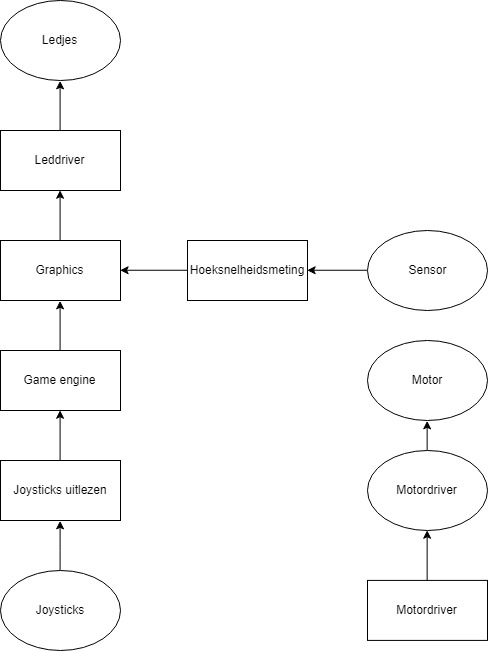
\includegraphics[width=0.8\textwidth]{img/structuur.jpg}
  \caption{Structuur van het microcontrollerprogramma}
  \label{fig:structuur}
\end{figure}


\subsection{Werking display}
Een schijf met gaten draait snel rond over LED's, verspreid in sectoren, zie figuur~\ref{fig:schijf}
Door de LED's op de gepaste momenten in en uit te schakelen
kan een zeer hoge resolutie bekomen worden rond het middelpunt.
In de radiale richting is de resolutie beperkt door het aantal LED's,
dit werd gekozen op 16 om de aansturing werkbaar te houden.

Met deze aanpak is het mogelijk om willekeurig de resolutie te kiezen
waarmee de hoek wordt beschreven. Hoe groter deze resolutie,
hoe meer pixels. Deze waarde werd gekozen op 1024.

\begin{figure}
  \centering
  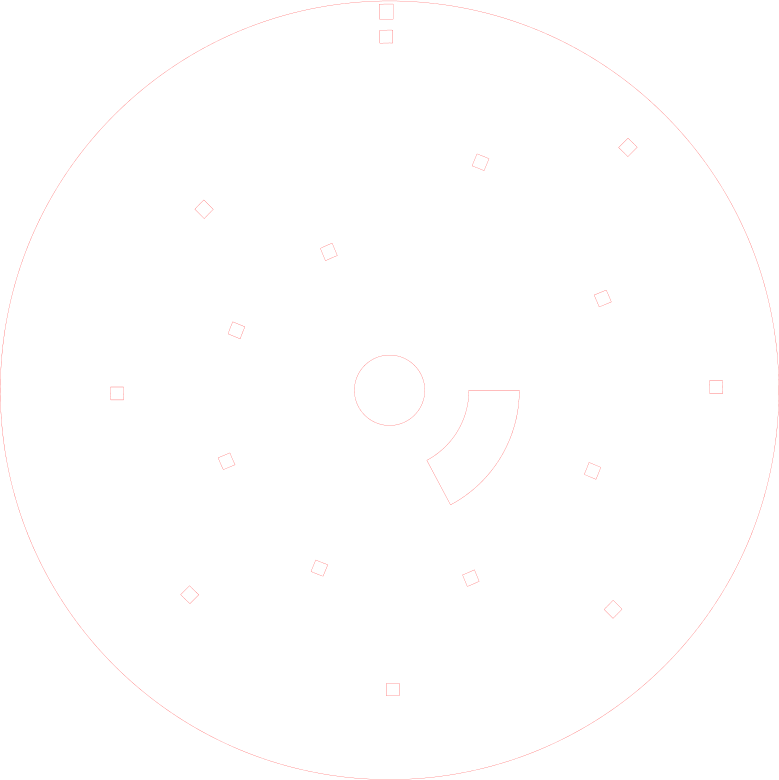
\includegraphics[width=0.6\textwidth]{img/schijf.png}
  \caption{Schema van de draaischijf}
  \label{fig:schijf}
\end{figure}

\subsection{Aansturing LED's}
De gebruikte LED's zijn ledstrips van het type \texttt{APA102}.
Deze kunnen vrij eenvoudig via SPI data ontvangen.
Elke LED krijgt een pakket bestaande uit 32 bits, zie
figuur~\ref{fig:ledpakket}.
Deze data moet byte per byte en bit per bit verzonden worden over één datalijn,
met een kloksignaal.

De ledstrip luistert naar nieuwe commando's na een startpakket
bestaande uit 32 0-bits. Vervolgens moet,
zoals zichtbaar op figuur~\ref{fig:ledcontrol},
een pakket per LED verstuurd worden gevolgd door
nogmaals 32 bits om te zorgen dat alle data ver genoeg doorgeschoven is.
De waarde van deze bits is onbelangrijk,
maar 0 is handig om te voorkomen dat er een LED op volle helderheid wit licht
geeft wanneer er niet naar elke LED gegevens worden gestuurd.

\begin{figure}
  \centering
  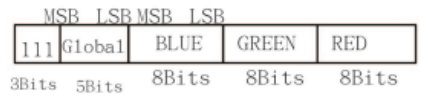
\includegraphics[width=0.6\textwidth]{img/ledpakket.png}
  \caption{Schema van een led-pakket}
  \label{fig:ledpakket}
\end{figure}

\begin{figure}
  \centering
  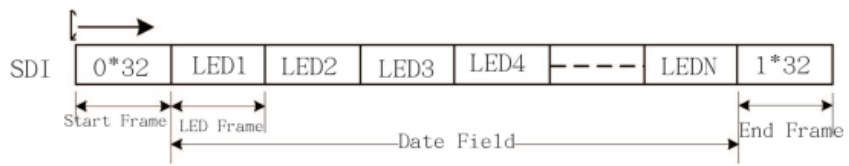
\includegraphics[width=0.8\textwidth]{img/ledcontrol.png}
  \caption{Schema van het aansturen van een ledstrip}
  \label{fig:ledcontrol}
\end{figure}

Er zijn twee mogelijke manieren om meerdere bytes te versturen over SPI,
via een blokkerende §while§-lus en via een interrupt.
Het is echter ook mogelijk om een interrupt te ontvangen wanneer een byte is
verzonden,
om vervolgens een volgende byte te verzenden. Op die manier kan CPU-tijd
uitgespaard worden, maar dit blijkt zeer lastig foutloos te implementeren.
Het spel gebruikt bijgevolg voorlopig nog de \emph{blocking} aanpak.

Het is handig om te weten wat de maximale frequentie is waarmee alle LED's
kunnen aangestuurd worden.
Hiervoor is het belangrijk te weten dat de microcontroller
een werkfrequentie heeft van \SI{16}{\mega\hertz}
en er maximaal 1 bit per 2 klokcycli kan verstuurd worden over SPI.
Er zijn 16 LED's, dit geeft een maximale frequentie van \SI{15625}{\hertz}.

\subsection{Timing LED's}
\label{sec:ledtiming}
De juiste LED's moeten op correcte momenten aan en uit geschakeld worden
om op de juiste plaats op de cirkel pixels op te laten lichten,
en niet te lang zodat de pixels geen lijnen worden.

Daartoe wordt voor elk weer te geven object in een snelle lus gecontroleerd of het
weer kan gegeven worden. Op de vergelijking van de hoek zit er een lichte marge,
zodat elk element zeker wordt weergegeven, ook al wordt het scherm niet snel
genoeg opnieuw getekend. Daartoe krijgt de functie zowel de tijd voor één volledige rotatie,
als de tijd sinds de schijf het nulpunt is gepasseerd als argumenten.
Daaruit kan namelijk de hoek waaronder de schijf staat bepaald worden.

\subsection{Fysieke constructie}
\TODO{Fysieke constructie}
De gehele constructie werd ontworpen in het CAD-pakket \textsc{Siemens NX 11} en
uitgesneden op een lasercutter, met uitzondering van enkele kleine stukken die
ge-3D-print\footnote{Dit is de correcte spelling volgens het Groene Boekje.} zijn.

De draaischijf bestaat uit dunne zwarte ABS, de behuizing uit MDF. De
reflectieve achtergrond en tussenschotten achter en tussen de LED's zijn uit een
vel wit plastic gesneden. Over de schijf zal een beschermende plaat transparant
acryl geplaatst worden, met een afbeelding van de aarde in het midden.

\subsection{Aansturing motor}
\TODO{Keuze timers en verder aanvullen}
De schijf draait rond met behulp van een brushless DC-motor uit een harde schijf.
Om deze aan te sturen is een speciale ESC-module\footnote{ESC: Electronic Speed Control} nodig.

Deze modules zijn ontworpen voor gebruik in quadcopters en verwachten bijgevolg
een speciale aansturing.
Het nodige signaal is een vorm van PWM, met een frequentie van 50 of
\SI{60}{\hertz}
en een pulsbreedte tussen 1 en \SI{2}{\milli\second}.
De PWM-modules die ingebouwd zitten in de microcontroller kunnen niet opereren
in deze frequenties en pulsbreedtelimieten,
het protocol werd dus volledig in software geïmplementeerd.
Zie figuur~\ref{fig:motorpwm} voor een beeld het geproduceerde signaal.

\begin{figure}
  \centering
  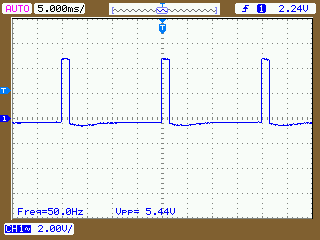
\includegraphics[width=0.6\textwidth]{img/scoopcontrolesc.png}
  \caption{Controlesignaal ESC}
  \label{fig:motorpwm}
\end{figure}

Een extra moeilijkheid is de opstartprocedure van de ESC.
De microcontroller moet opgestart zijn en een signaal sturen dat overeen komt
met \SI{0}{\percent} motorvermogen wanneer de ESC stroom krijgt en wordt
ingeschakeld. De ESC produceert dan een serie tonen, gevolgd door een langere
toon wanneer het signaal herkend wordt. Daarna kan de motor aangestuurd worden
en het vermogen verhoogd, liefst langzaam gezien het hoge gewicht van de draaischijf.
Uiteindelijk zal de ESC een driefasig signaal naar de motor sturen, zoals
zichtbaar in figuur~\ref{fig:motoresc}.

\begin{figure}
  \centering
  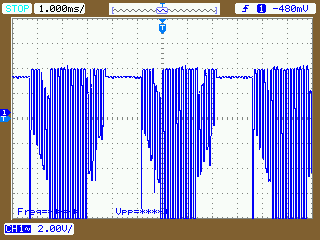
\includegraphics[width=0.6\textwidth]{img/scoopesc.png}
  \caption{Vermogenssignaal naar de motor}
  \label{fig:motoresc}
\end{figure}

Deze procedure maakt het moeilijk om microcontroller en ESC op één voeding te
laten werken. Door de grote stroom is het ook lastig om bijvoorbeeld de ESC te
schakelen met een transistor. Voorlopig moet de ESC manueel in de stekker
gestoken worden. De driver wacht daartoe even met het opstarten van de motor,
aangezien de stekker pas mag ingeplugd worden wanneer het stuursignaal reeds
aanwezig is.

\subsection{Toerenteller schijf}
Op de schijf zit een optische sensor, die registreert wanneer een gaatje
passeert. De microcontroller telt nauwkeurig op welk moment dit gebeurt,
zodat afgeleid kan worden hoe snel de schijf draait.
\TODO{Info toerenteller}

\subsection{Joysticks}
De beide joysticks zijn relatief eenvoudig om uit te lezen.
Ze bestaan telkens uit vier \emph{NO} schakelaars, één per richting.
Aangezien elke joystick op een aparte \emph{port} van de microcontroller
aangesloten is, kan met een simpele §NOT§ operatie en enkele bitshifts een
consistente weergave gegenereerd worden, met 1 bit per richting die hoog is
wanneer de schakelaar actief is. Hiertoe moeten ook de pullups geactiveerd
worden. De driver voor de joysticks controleert ook welke schakelaars sinds de
laatste tick actief zijn geworden, en slaat deze apart op.

Enkele gemaksfuncties werden toegevoegd om uit deze bitweergave te bepalen of
een gekozen richting actief is.

\subsection{Game engine}
De game engine werkt op een relatief eenvoudig principe.
Op regelmatige basis wordt de functie §uint8_t tick(uint16_t time_since_zero)§
opgeroepen, deze voert enkele stappen uit:
\begin{enumerate}
  \item \emph{Tick alle entities}\footnote{Entities zijn bijvoorbeeld kogels en
        spelers}, entities hebben een §tick()§ functie,\\
    bijvoorbeeld §player_tick(Player *p)§, die ervoor zorgt dat de entity zich
    verplaatst volgens zijn snelheid en eventueel reageert op invoer.

  \item \emph{Controleer voor botsingen}, in deze stap wordt getest of er
    kogels een schip geraakt hebben, en eventueel levens van deze speler worden
    afgenomen.

  \item \emph{Check voor het einde van het spel} door te controleren of beide
    spelers nog in leven zijn. Dit bepaalt de returnwaarde van deze functie,
    §true§ wanneer het spel moet verder gaan, anders §false§.
\end{enumerate}

Deze functie wordt aan \SI{30}{\hertz} opgeroepen, met behulp van
\texttt{Timer/Counter0} in \emph{CTC} mode. De counter geeft dan een interrupt
telkens een ingestelde waarde wordt bereikt en begint vervolgens weer vanaf nul
te tellen. Voorlopig telt de counter tot \num{255}, indien mogelijk kan dit
later verlaagd worden om het spel sneller te maken.
De 8-bits resolutie is meer dan genoeg om een vrij
groot bereik van mogelijke frequenties te bereiken met de prescaler op de
maximale waarde van $1024$.
Apart daarvan wordt zo snel mogelijk de §render(uint8_t time_since_zero)§
functie opgeroepen, die de LED's schakelt.

\section{Problemen}
\subsection{ESC}
Na een eerste poging bleek dat de ESC de motor niet kon laten draaien.
De motor gaf wat schokjes en de ESC produceerde niet de gewenste opstarttonen.
Na de massakabel van de motor los te maken bleek alles correct te functioneren.
Het is onbekend waarom dit een probleem gaf.

\subsection{Light bleed}
Soms lichtten er pixels vaag op die niet moesten oplichten,
dit bleek te zijn doordat er soms twee gaten over dezelfde sector hingen, wat
mogelijk was omdat de scheiding tussen sectoren bestaat uit dun, reflectief
plastic.

Er werd besloten om de verticale resolutie te verlagen, zodat de sectoren op de
draaischijf groter worden, maar de sectoren met de LED's ongewijzigd te houden.
Een andere optie zou zijn om de wanden tussen de sectoren dikker te maken.

\section{Openstaande Problemen}
Er is nog wat werk aan de fysieke constructie van de schijf en we twijfelen nog
over het aantal sectoren. Een groot deel van de code, zoals de \emph{game
  engine} en de driver voor LED-timing, is dus nog niet getest.
Dit testen en debuggen zal waarschijnlijk nog vrij veel tijd innemen.
Verder zijn er nog enkele verbeteringen te maken in de \emph{game engine},
zo wordt er nog geen melding gegeven wanneer een speler sterft en kan het spel
niet herstart worden zonder de microcontroller te resetten.
Het spel begint ook van zodra de controller opstart, in plaats van wanneer de
spelers klaar zijn. Dit is geen wenselijke werking.

\section{Taakverdeling en Samenwerking}
De motordriver werd geschreven door Marieke. Zij schreef ook de code die voor de
juiste timing zorgt en de optische sensor uitleest.

De game engine en aansturing van LED's werd gedaan door Stef,
net zoals uitlezen van Joysticks en debugfunctionaliteit.

Ontwerp en constructie van de behuizing is door Marieke.

Scoutt was verantwoordelijk voor een deel van het bestand \texttt{Pins},
dat bijhoudt welke pins op de microcontroller in gebruik zijn door welk systeem.
Hij is ook verantwoordelijk voor commit
\href{https://github.com/Epse/MCU_Project_PlanetFight/commit/142748a7c49a4552b92dfe5613a2f1f7b7a7eb75}{\texttt{142748a:}~\emph{Nuttelose
    comment} (sic.)}.

Onze samenwerking gebeurt via Git en
GitHub\footnote{\url{https://github.com/Epse/MCU_Project_PlanetFight}}. Taken worden
verdeeld via \emph{issues} op GitHub. Iedereen werkt aan een apart deel van de
code of de hardware, die regelmatig samen worden gezet.

\section{Conclusie en Toekomstig Werk}

\end{document}
